\documentclass[12pt, fleqn]{article}

\usepackage{../../../template/template}
\usepackage{../../../template/KillContents}
 
\begin{document}
    \tableofcontents
    \newpage
    \begin{lect} {11.10.19}
        \section{Условные экстремумы}
        \[u = f(x_1, ..., x_n) \text{ при усл } \begin{cases}
            \Phi_1 (x_1, ..., x_n) = 0\\
            \vdots\\
            \Phi_m (x_1, ..., x_n) = 0
        \end{cases} \q m < n\]
        \begin{enumerate}
            \item Точка недифф-ти $f$ или $\Phi_i$
            \item $\rk \Phi' < m$
            \item $\LL = f(x_1, ..., x_n) - \lambda_1 \Phi_1 (x_1, ..., x_n) - 
                \lambda_2 \Phi_2 (x_1, ..., x_n) - ... -\lambda_m \Phi_m(x_1, ..., x_n)$
        \end{enumerate}
            
        \[\Phi' = \begin{pmatrix}
            \frac{\partial \Phi_1}{\partial x_1} & ... & \frac{\partial \Phi_1}{\partial x_n}\\
            \vdots & & \vdots\\
            \frac{\partial \Phi_m}{\partial x_1} & ... & \frac{\partial \Phi_m}{\partial x_n}
        \end{pmatrix} \qq m \times n\]
        Точка экстремума удовлетворяет системе уравнений:
        \[\begin{cases}
                \frac{\partial \LL}{\partial x_1} = 0\\
                \vdots\\
                \frac{\partial \LL}{\partial x_n} = 0\\
                \Phi_1(x_1, ..., x_n) = 0\\
                \vdots\\
                \Phi_m(x_1, ..., x_n) = 0
        \end{cases} \qq m + n \text{ уравнений } \q \]
        \[m + n \text{ неизвестных} \q x_1, ..., x_n, \lambda_1, ..., \lambda_m\]

        \begin{Task}[1]
            \[f(x, y) = \frac{x}{a} + \frac{y}{b} \qq a, b > 0 \text{ при усл. } x^2 + y^2 = 1 \rla \underbracket{x^2 + y^2 - 1 = 0}_{\Phi} \qq M \]
            \[\Phi' = \begin{pmatrix}
                2x & 2y
            \end{pmatrix} \qq \text{1 ур-е } \Ra \text{1 строка в матрице}\]
            \[\rk \Phi' < 1 \Ra \rk \Phi'  = 0  \q\Ra \begin{cases}
                    x = 0\\
                    y = 0
            \end{cases} \cancel{\in } M\]
            \[\forall (x, y) \in M \qq \rk \Phi' = 1\]
            \[\LL = \frac{x}{a} + \frac{y}{b} - \lambda(x^2 + y^2 - 1)\]
            \[\begin{cases}
                \LL'_x = \frac{1}{a} - 2\lambda \cdot x = 0 \Ra \lambda \neq 0 \qq &x = \frac{1}{2a\lambda}\\
                \LL'_y = \frac{1}{b} - a\lambda \cdot y = 0 \Ra &y = \frac{1}{2b\lambda}\\
                x^2 + y^2 = 1       
            \end{cases}\] 
            \[\frac{1}{4a^2\lambda^2} + \frac{1}{4b^2\lambda^2} = 1\]
            \[\frac{b^2 + a^2}{4a^2b^2\lambda^2} = 1\]
            \[a^2 + b^2 = 4a^2b^2 \lambda^2\]
            \[\lambda = \pm \frac{\sqrt{a^2 + b^2}}{2ab}\]
            \[1.\begin{cases}
                x = \frac{1 \cdot 2 ab}{2a \sqrt{a^2 + b^2}} = \frac{b}{\sqrt{a^2 + b^2}}\\
                y = \frac{a}{\sqrt{a^2 + b^2}}\\
                \lambda = +\frac{\sqrt{a^2 + b^2}}{2ab}
            \end{cases}\]
            \[2.\begin{cases}
                x = -\frac{b}{\sqrt{a^2 + b^2}}\\
                y = - \frac{a}{\sqrt{ a^2 + b^2}}\\
                \lambda = -\frac{\sqrt{a^2 + b^2}}{2ab}
            \end{cases}\]  
            Выясним, что будет в этих точках
            \[\LL_{x^2}'' = -2\lambda\]
            \[\LL_{xy}'' = 0 \]
            \[\LL_{y^2}'' = -2\lambda\]
            \[\begin{pmatrix}
                -2\lambda & 0\\
                0   & -2 \lambda
            \end{pmatrix} \qq \Delta_1 = 2\lambda \q \Delta_2 = 4\lambda^2\]
            \[\begin{matrix}
                \text{для } & 1. & - & + & \max\\
                            & 2. & + & + & \min
            \end{matrix}\]
        \end{Task}

        \begin{Task}[2]
            \[u = x^2 + y^2 + z^2\]
            \[\frac{x^2}{a^2} + \frac{y^2}{b^2} + \frac{z^2}{c^2} = 1 \qq a > b > c > 0\]
            \[\frac{x^2}{a^2} + \frac{y^2}{b^2} + \frac{z^2}{c^2} - 1 = 0\]
            \[\Phi' = \begin{pmatrix}
                \frac{2x}{a^2} & \frac{2y}{b^2} & \frac{2z}{c^2}
            \end{pmatrix}\]
            \[\rk \Phi' = 0  \Ra \q x = y = z = 0 \qq (0, 0, 0) \cancel{\in } M\]
            \[\LL = x^2 + y^2 + z^2 - \lambda(\frac{x^2}{a^2} + \frac{y^2}{b^2} + 
            \frac{z^2}{c^2} - 1)\]
            \[\begin{cases}
                \LL_x' = 2x - \frac{2x\lambda}{a^2} = 0 
                \Ra x(1 - \frac{\lambda}{a^2}) = 0\\
                \LL'_y = 2y - \frac{2y\lambda}{b^2} = 0 
                \Ra y(1 - \frac{\lambda}{b^2}) = 0\\
                \LL'_z = 2z - \frac{2z\lambda}{c^2} = 0
                \Ra z(1 - \frac{\lambda}{c^2}) = 0\\
                \frac{x^2}{a^2} + \frac{y^2}{b^2} + \frac{z^2}{c^2} = 1
            \end{cases}\]
            \[1 - \frac{\lambda}{b^2} = 0 \Ra \lambda = b^2\]
            \[x = z = 0 \qq y \pm b\]
            \[1 - \frac{\lambda}{c^2} = 0 \Ra \lambda = c^2\]
            \[x = y = 0 \qq z = \pm c\]
            \[1 - \frac{\lambda}{a^2} = 0\]
            \[\lambda = a^2  \qq 1 - \frac{a^2}{b^2} \neq 0\]
            \[\Ra y = 0\]
            \[1 - \frac{a^2}{c^2} \neq 0 \Ra z = 0\]
            \[\Ra \frac{x^2}{a^2} = 1\]
            \[\begin{cases}
                x = \pm a\\
                y = 0\\
                z = 0\\
                \lambda = a^2
            \end{cases}\]
            \[\text{6 решений } \begin{matrix}
                \begin{pmatrix}
                    \pm a & 0 & 0 & a^2\\
                \end{pmatrix} \q
                \begin{pmatrix}
                    0 & \pm b & 0 & b^2\\
                \end{pmatrix}\q
                \begin{pmatrix}
                    0 & 0 & \pm c & c^2
                \end{pmatrix}
            \end{matrix}\]
            \[\begin{pmatrix}
                2 - \frac{2\lambda}{a^2} & 0 & 0\\
                0 & 2 - \frac{2\lambda}{b^2} & 0\\
                0 & 0 & 2 - \frac{2\lambda}{c^2}
            \end{pmatrix}\]
            \[\Delta_1 = 2 - \frac{2\lambda}{a^2} = 2(1- \frac{\lambda}{a^2})\]
            \[\Delta_2 = 4(1 - \frac{\lambda}{a^2})(1 - \frac{\lambda}{b^2})\]
            \[\Delta_3 = 8(1 - \frac{\lambda}{a^2})(1 - \frac{\lambda}{b^2})
            (1 - \frac{\lambda}{c^2})\]
            \begin{enumerate}
                \item $\lambda = a^2 \qq 0, \ 0,\  0$
                \item $\lambda = b^2 \qq 1 - \frac{b^2}{a^2} > 0, \ 0, \ 0$
                \item $\lambda = c^2 \qq 1 - \frac{c^2}{a^2} > 0, \ 
                    (1 - \frac{c^2}{a^2})(1 - \frac{c^2}{b^2}) > 0, \ 0$
            \end{enumerate}
            Но у нас $2$ независимые переменные
            \[d^2\LL = 2(1 - \frac{\lambda^2}{a^2})(dx)^2 + 
            2(1 - \frac{\lambda}{b^2})(dy)^2 + 2(1 - \frac{\lambda}{c^2})(dz)^2\]
            \[\frac{2x}{a^2}dx + \frac{2y}{b^2}dy + \frac{2z}{c^2}dz = 0\]
             - линейная однородная система относительно диф-лов
            \[dx, dy, dz \text{ - зависимы между собой}\]
            \[\text{В точке } \begin{pmatrix}
                \pm a, & 0, & 0, & a^2
            \end{pmatrix} \text{ - максимум}\]
            \[\frac{\pm 2a}{a^2}dx = 0 \Ra dx \equiv 0\]
            \[d^2 \LL = 2(1 - \frac{a^2}{b^2})(dy)^2 + 2(1 - \frac{a^2}{c^2})(dz)^2\]
            \[\begin{pmatrix}
                2(1 - \frac{a^2}{b^2}) & 0\\
                0 & 2(1 - \frac{a^2}{c^2})
            \end{pmatrix} \qq \begin{matrix}
                \Delta_1 =& 2(1 - \frac{a^2}{b^2}) < 0\\
                \Delta_2 =& 4 (1 - \frac{a^2}{b^2})(1 - \frac{a^2}{c^2}) > 0\\
                - \q +  &\ul{\text{ максимум }}
            \end{matrix}\]
            \[\text{В точке } \begin{pmatrix}
                0, & \pm b, & 0, & b^2
            \end{pmatrix} \text{ нет экстремума}\]
            \[\pm \frac{2b}{b^2}dy = 0 \Ra dy = 0\]
            \[d^2\LL = 2(1 - \frac{b^2}{a^2})(dx)^2 + 2(1 - \frac{b^2}{c^2})(dz)^2\]
            \[\begin{pmatrix}
                2(1 - \frac{b^2}{a^2}) & 0\\
                0 & 2(1 - \frac{b^2}{c^2})
            \end{pmatrix} \qq \begin{matrix}
                \Delta_1 =& 2(1 - \frac{b^2}{a^2}) > 0\\
                \Delta_2 =& 4(1 - \frac{b^2}{a^2})(1 - \frac{b^2}{c^2}) < 0\\
                + \q - & \ul{\text{ нет экстремума}}
            \end{matrix}\]
            \[\text{В точке } \begin{pmatrix}
                0, & 0, & \pm c, & c^2
            \end{pmatrix} \text{ - минимум}\]
            \[\pm \frac{2c}{c^2}dz = 0 \Ra dz = 0\]
            \[d^2\LL = 2(1 - \frac{c^2}{a^2})(dx)^2 + 2(1 - \frac{c^2}{b^2})(dy)^2\]
            \[\begin{pmatrix}
                2(1 - \frac{c^2}{a^2}) & 0\\
                0 & 2(1 - \frac{c^2}{b^2})
            \end{pmatrix} \qq \begin{matrix}
                \Delta_1 =& 2(1 - \frac{c^2}{a^2}) > 0\\
                \Delta_2 =& 4(1 - \frac{c^2}{a^2})(1 - \frac{c^2}{b^2}) > 0\\
                + \q + & \ul{\text{ минимум}} 
            \end{matrix}\]
        \end{Task}

        \begin{Task}[3]
            \[u = xy + yz\]
            \[\begin{cases}
                x^2 + y^2 = 2\\
                y + z = 2
            \end{cases} \qq \begin{cases}
            x^2 + y^2 - 2 = 0 & \q M\\
                y + z - 2 = 0
            \end{cases}\]
            \[\Phi' = \begin{pmatrix}
                2x & 2y & 0\\
                0 & 1 & 1
            \end{pmatrix} \qq \rk \Phi' < 2\]
            \[\Delta_1 = \begin{vmatrix}
                2x & 2y\\
                0 & 1
            \end{vmatrix} = 2x\]
            \[\Delta_2 = \begin{vmatrix}
                2x & 0\\
                0 & 1
            \end{vmatrix} = 2x\]
            \[\Delta_3 = \begin{vmatrix}
                2y & 0\\
                1 & 1
            \end{vmatrix} = 2y\]
            \[\Delta_1 = \Delta_2 = \Delta_3 = 0 \Ra \begin{cases}
                x = 0\\
                y = 0
            \end{cases} \text{ противоречие с } x^2 + y^2 = 2\]
            \[\forall (x, y) \in M \qq \rk \Phi' = 2\]
            \[\LL = xy + yz - \lambda_1(x^2 + y^2 - 2) - \lambda_2(y + z - 2)\]
            \[\begin{cases}
                \LL_x' = y - 2\lambda_1x &= 0\\
                \LL_y' = x + z - 2\lambda_1y - \lambda_2 &= 0\\
                \LL_z' = y - \lambda_2 &= 0\\
                x^2 + y^2 &= 2\\
                y + z &= 2
            \end{cases}\]
            \[\Ra x \neq 0 \q \lambda_1 = \frac{y}{2x}\]
            \[x = 0 \Ra y = 0 \text{ - противореч с } x^2 + y^2 = 2\]
            \[\rla \begin{cases}
                \lambda_1 = \frac{y}{2x}\\
                \lambda_2 = y\\
                x + z - \frac{y^2}{x} - y = 0\\
                x^2 + y^2 = z\\
                z = 2 - y
            \end{cases} \rla \begin{cases}
                \lambda_1 = \frac{y}{2x}\\
                \lambda_2 = y\\
                x + 2 - y - \frac{y^2}{x} - y = 0\\
                x^2 + y^2 = 2\\
                z = 2 - y
            \end{cases} \os{x \neq 0}{ \rla}\]
            \[\rla \begin{cases}
                \lambda_1 = \frac{y}{2x}\\
                \lambda_2 = y\\
                x^2 + 2(1 - y)x - y^2 = 0\\
                x^2 = 2 - y^2\\
                z = 2 - y
            \end{cases} \rla \begin{cases}
                \lambda_1 = \frac{y}{2x}\\
                \lambda_2 = y\\
                2 - 2y^2 + 2(1 - y)x = 0\\
                x^2 = 2 - y^2\\
                z = 2 - y
            \end{cases} \rla\]
            \[\rla \begin{cases}
                \lambda_1 = \frac{y}{2x}\\
                \lambda_2 = y\\
                (1 - y)(1 + y) + x(1 - y) = 0\\
                x^2 = 2 - y^2\\
                z = 2 - y
            \end{cases}\]
            \[(1 - y)(1 + y + x) = 0\]

            \[1. \q y = 1\]
            \[x^2 = 1 \Ra x = \pm 1\]
            \[z = 2 - y = 1\]
            \[\lambda_2 = 1\]
            \[\lambda_1 = \pm \frac{1}{2}\]
            \[(1) \begin{cases}
                x = 1\\
                y = 1\\
                z = 1\\
                \lambda_1 = \frac{1}{2}\\
                \lambda_2 = 1
            \end{cases} \qq (2) \begin{cases}
                x = -1\\
                y = 1\\
                z = 1\\
                \lambda_1 = -\frac{1}{2}\\
                \lambda_2 = 1
            \end{cases}\]

            \[2. \q 1 + y + x = 0\]
            \[x = -1 - y\]
            \[(-1 - y)^2 = 2 - y^2 \qq y = \frac{-1 \pm \sqrt{3}}{2}\]
            \[y^2 + 2y + 1 = 2 - y^2 \qq z = 1 - \frac{-1 \pm \sqrt{3}}{2} = 
            \frac{-2 + 1 \mp \sqrt{3}}{2}\]
            \[2y^2 + 2y - 1 = 0\]
            \[(3)\begin{cases}
                x = \frac{ -1 - \sqrt{3}}{2}\\
                y = \frac{ -1 + \sqrt{3}}{2}\\
                z = \frac{5 - \sqrt{3}}{2}\\
                \lambda_1 = ...\\
                \lambda_2 = ...
            \end{cases} \qq (4) \begin{cases}
                x = \frac{-1  +\sqrt{3}}{2}\\
                y = \frac{-1 - \sqrt{3}}{2}\\
                z = \frac{5 + \sqrt{3}}{2}\\
                \lambda_1 = ...\\
                \lambda_2 = ...
            \end{cases}\]
            \[\begin{pmatrix}
                -2 \lambda_1 & 1 & 0\\
                1 & -2\lambda_1 & 1\\
                0 & 1 & 0
            \end{pmatrix} \qq \begin{matrix}
                \Delta_1 = -2\lambda_1\\
                \Delta_2 = 4\lambda_1^2 - 1\\
                \Delta_3 = -1 \begin{vmatrix}
                    -2 \lambda_1 & 0\\
                    1 & 1
                \end{vmatrix} = 2\lambda_1
            \end{matrix}\]
            В $(1)$\q -\ 0\ + \q экстр. нет?\\
            В $(2)$\q +\ 0\ - \q экстр. нет?\\
            \[d^2\LL = (-2 \lambda_1)(dx)^2 + 2dxdy + (-2\lambda_1)(dy)^2 + 2dydz\]
            \[\begin{cases}
                x^2 + y^2 = 2\\
                y + z = 2
            \end{cases} \qq \begin{cases}
                2xdx + 2ydy = 0\\
                dy + dz = 0
            \end{cases}\]
            \[\text{В точке } \begin{pmatrix}
                1,& 1,& 1
            \end{pmatrix}\]
            \[\begin{cases}
                dx + dy = 0\\
                dy + dz = 0
            \end{cases} \qq \begin{cases}
                dx = -dy\\
                dz = -dy
            \end{cases}\]
            \[d^2\LL = (-dy)^2 + 2(-dy)dy - (dy)^2 + 2dy(-dy) = (-6)(dy)^2\]
            \[\begin{pmatrix}
                -6
            \end{pmatrix} \text{ матрица из одного элемента}\] 
            \[\Delta_1 < 0 \qq - \max\]
            \hline
            \[\text{В точке }\begin{pmatrix}
                1, & 1, & 1
            \end{pmatrix} \qq \lambda = - \frac{1}{2}\]
            \[\begin{cases}
                -dx + dy = 0\\
                dy + dz = 0
            \end{cases} \qq \begin{cases}
                dx = dy\\
                dz = -dy
            \end{cases}\]
            \[d^2 \LL = 1 \cdot (dy)^2 + 2dydy + 1 \cdot (dy)^2 + 2dy \cdot (-dy) = 2 (dy)^2\]
            \[\begin{pmatrix}
                2
            \end{pmatrix} \qq \Delta_1 > 0 \qq \Ra \min\]
            \[\begin{pmatrix}
                -1, & 1, & 1
            \end{pmatrix} \qq - \min\]
            
        \end{Task}
        
        \section{наиб. и наим. значения функций от нескольких перем.}
        \begin{Definition}
            \begin{figure}[H]
                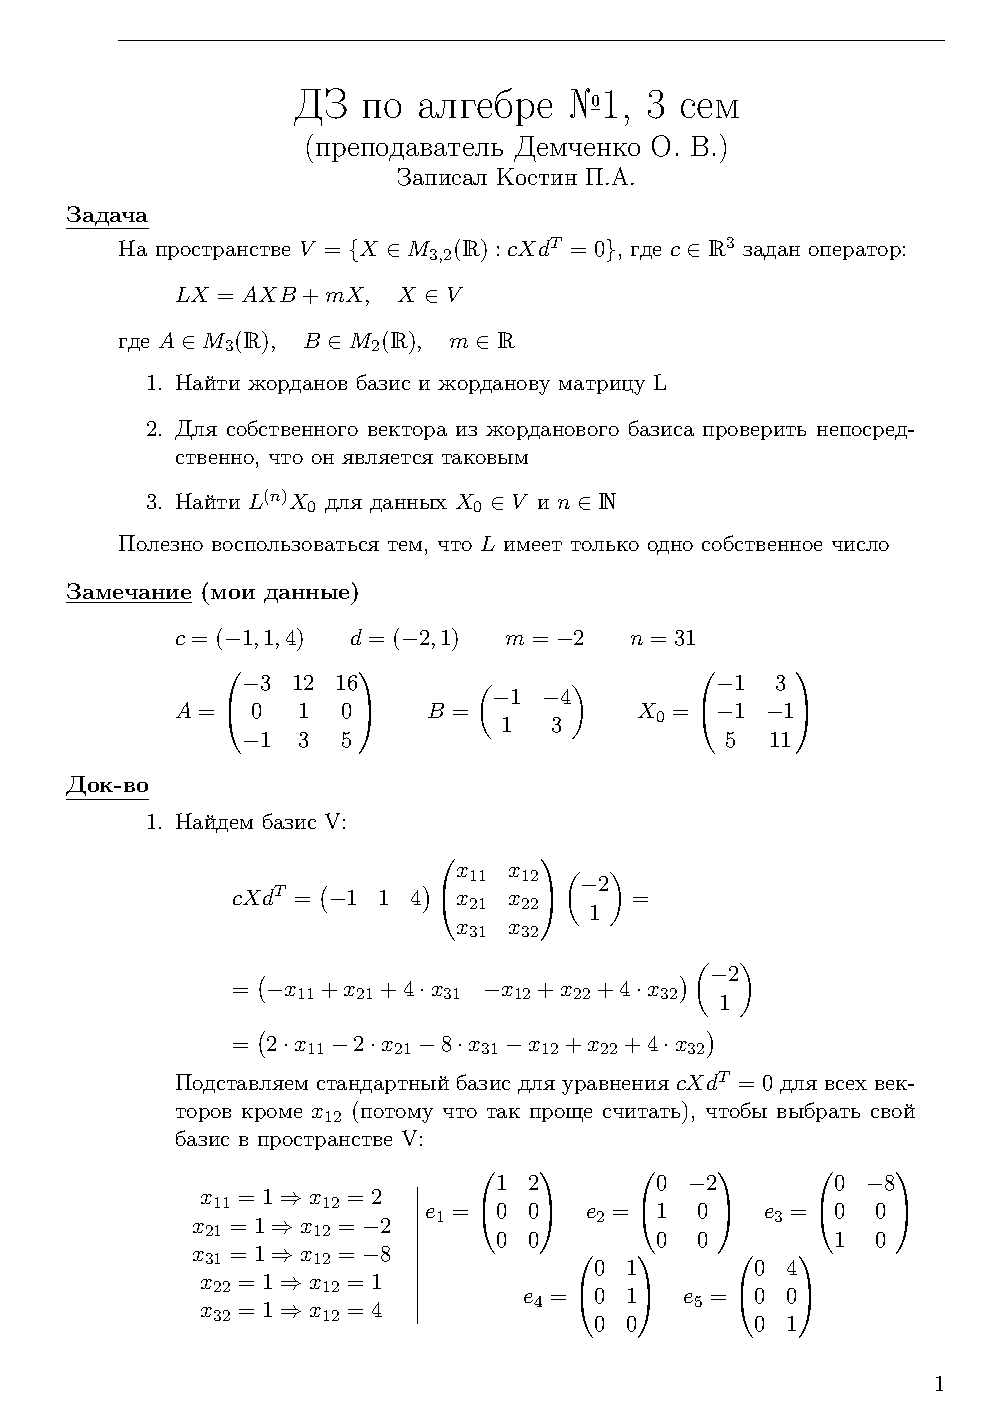
\includegraphics[width=10cm]{pics/1.png}
                \centering
            \end{figure}
            \[\text{ наиб и наим знач. ф. } u = f(x, y, z) \text{ на } E\]
            \begin{enumerate}
                \item внутри $E$ \Ra $\begin{cases}
                    
                \end{cases}$
            \end{enumerate}
        \end{Definition} 
    \end{lect} 

    \begin{lect}{2019-10-25}
    
    \section{Неявные функции. Вычисл. их диф-лов, производных. Разложения неявных 
    функций по ф-ле Тейлора}
    
    \begin{reminder}
        неявные ф-ии задаются системой ур-й
    \end{reminder}

    \[F_i \in C^1 (G)\]
    \[\begin{cases}
        F_1(x_1, ..., x_m, y_1, ..., y_n) = 0\\
        ...\\
        F_n(x_1, ..., x_m, y_1, ..., y_n) = 0
    \end{cases} \os{?}{\rla} \begin{cases}
    y_1 = f_1(x_1, ..., x_m)\\
    ...\\
    y_n = f_n(x_1, ..., x_m)
    \end{cases}\]
    \[m + n \text{ - перем. } \q n - \text{ ур-ний}\]

    \begin{theorem}
        Если сис-ма удовлетв-ся в точке $(x_1^0, ..., x_m^0, y_1^0, ..., y_n^0)$ и в этой 
        точке 
        \[\begin{vmatrix}
            \frac{\partial F_1}{\partial y_1} & ... & \frac{\partial F_1}{\partial y_n}\\
            \vdots\\
            \frac{\partial F_n}{\partial y_n} & ... & \frac{\partial F_n}{\partial y_n}
        \end{vmatrix} \neq 0\]
        То в окрестн. точки $(x_1^0, ..., x_m^0, y_1^0, ..., y_n^0)$ система однозн. 
        разрешима и $f_k \in C^1(u(x_1^0, ..., x^0_m)) $\\
        \\
        Если $F_i \in C^r(G)$ \qq $\Ra f_k \in C^r(u(x_1^0, ..., x_m^0))$\\
        Вычислим диф-лы от каждого ур-я
        \[\begin{cases} \displaystyle 
            \frac{\partial F_1}{\partial x_1} dx_1 + ... + \frac{\partial F_1}{
            \partial x_m}dx_m + \frac{\partial F_1}{\partial y_1}dy_1 + ... +
            \frac{\partial F_1}{\partial y_n}dy_n = 0\\\\ \displaystyle 
            \frac{\partial F_2}{\partial x_1} dx_1 + ... + \frac{\partial F_2}{
            \partial x_m}dx_m + \frac{\partial F_2}{\partial y_1}dy_1 + ... +
            \frac{\partial F_2}{\partial y_n}dy_n = 0\\
            ...\\\\\displaystyle 
            \frac{\partial F_n}{\partial x_1} dx_1 + ... + \frac{\partial F_n}{
            \partial x_m}dx_m + \frac{\partial F_n}{\partial y_1}dy_1 + ... +
            \frac{\partial F_n}{\partial y_n}dy_n = 0
        \end{cases}\]
        Линейная однородная система относительно $dy_1, .., dy_n$\\
        $\Ra$ система однозначно разрешима (т.к. )
        \[dy_1 = \underbracket{...}_{\to \frac{\partial F_1}{\partial x_1}} dx_1 + 
            \underbracket{...}_{\to \frac{\partial F_1}{\partial x_2}} dx_2 + 
            ... +
            \underbracket{...}_{\to \frac{\partial F_1}{\partial x_m}} dx_m + 
        \]
        \[...\]
        \[dy_n = ... dx_1 + ... dx_2 + ... + ... dx_m\]
    \end{theorem}

    \begin{Task}[1]
        \[F = z^3 - 3xyz - 1 = 0 \rla z = z(x, y)\]
        \[x_0 = 0, y_0 = 1 \Ra z_0 = 1\]
        \[\text{Хотим найти } \frac{\partial z}{\partial x};\q \frac{\partial z}
        {\partial y};\q \frac{\partial^2 z}{\partial x^2};\q \frac{\partial^2 z}
        {\partial x
    \partial y}... \qq (\text{В том числе в точке } (0, 1))\]
        \[dF = -3yzdx - 3xzdy + (3z^2 - 3xy)dz = 0\]
        \[3z_0^2 - 3x_0y_0 = 3 \neq 0\]
        \[\Ra dz = + \frac{yz}{z^2 - xy}dx + \frac{xz}{z^2 - xy}dy\]
        \[\Ra \frac{\partial z}{\partial x} = + \frac{yz}{z^2 - xy}\]
        \[\frac{\partial z}{\partial y} = + \frac{xz}{z^2 - xy}\]
        \[x_0 = 0\]
        \[y_0 \Ra z_0 = 1\]
        \[\frac{\partial z}{\partial x}(0, 1) = 1\]
        \[\frac{\partial z}{\partial y}(0, 1) = 0\]
        hint: Если нужны только в конкрет. точке, то проще подставить точку в ур-е
        \[-3 \cdot 1 \cdot 1dx -3 \cdot 0 \cdot 1 dy + 3( 1 - 0 \cdot 1)dz = 0\]
        \[\Ra dz = dx = 1\cdot dx + 0 \cdot dy\]
        \[-yzdx -xzdy + (z^2 - xy)dz = 0\]
        \[hint: \q d(P \cdot Q) = P \cdot dQ + Q \cdot dP\]
        \[d(-yz)dx + (-yz)d^2x + d(-xz)dy + (-xz)d^2y + d(z^2 - xy)dz + (z^2 -xy)d^2z
        = 0\]
        \[x, y \text{ - нез. перем. (т.к. $z$ - функция )} \Ra d^2x, d^2y = 0\]
    \end{Task}

    \begin{Task} [3]
        \[(F)(\us{1}{x}, \ \us{2}{x + y}, \  \us{3}{x + y + z}))'_x = 0\]
        \[z = z(x, y) \qq \frac{\partial z}{\partial x} - ? \q
         \frac{\partial ^2 z}{\partial x^2} - ?\]
         \[F'_1 \cdot (x)'_x + F'_2 \cdot (x + y)'_x + F_3' \cdot (x + y + z)'_x = 0\]
         \[F'_1 \cdot 1 + F_2' \cdot 1 + F'_3 \cdot (1 + z_x') = 0\]
         \[F'_3 \cdot z'_x = -F_1' - F'_2  - F'_3 \Ra z'_x = -\frac{F'_1 + F'_2}{F'_3}
         - 1\]
         \[(F_1'(\us{1}{x}, \us{2}{x + y}, \us{3}{x + y + z}))'_x = 
         F''_{11} \cdot (x)'_x + F''_{12} \cdot (x + y)'_x + F_{13}'' \cdot 
         (x + y + z)'_x =\]
         \[ = F''_{11} + F''_{12} + F''_{13} + F''_{13} \cdot z'_x\]
         \[(F'_3 \cdot z'_x)'_x = (F_3')'_{x} \cdot z'_x + F'_x \cdot z''_{xx}  \]
         \[F''_{11} + F_{12}'' + F_{13}'' + F''_{13} \cdot z'_x  + 
         F''_{21} + F''_{22} + F''_{23} + F''_{23} \cdot z'_x + 
         F''_{31} + F''_{32} + F''_{33} + F''_{33} \cdot z'_x + \]
         \[+ (F''_{31} + F''_{32} + F''_{33} + F''_{33}\cdot z'_x) \cdot z'_x  + 
         F'_3 \cdot z''_{xx} = 0 \]
         \[F''_{11} + 2F''_{12} + 2F''_{13} + F''_{22} + 2F''_{23} + F''_{33} + 
         (2F''_{13} + 2F''_{23} + 3F''_{33}  ) \cdot z'_x + F''_{33} \cdot(z'_x)^2 + 
         F'_3 \cdot z''_{xx} = 0 \]
         \[F'_3 \cdot z''_{xx} = -F_{11}'' - 2F''_{12} - ... - 
         (2F''_{13} + 2F''_{23} + 2F''_{33}) \cdot (- \frac{F'_1 + F'_2}{F_3'} - 1) - \]
         \[ - F''_{33} (-\frac{F'_1 + F'_2}{F'_3} - 1)^2 \]
         \[z''_{xx} \text{ - из ур=я} \]
         \[z''_{xx} = - (\frac{F'_1  + F'_2}{F'_3})'_x \]
    \end{Task}

    \begin{Task}[4 Замена переменных в дифф. ур]
        \[F(x, y, z, \frac{\partial z}{\partial x}, \frac{\partial z}{\partial y}, 
        \frac{\partial ^2 z}{\partial x^2}, \frac{\partial^2 z}{\partial x \partial z}, ...) = 0\]
        \[z = z(x, y)\]
        \[\text{новые переменные } u, v \qq w(u, v) \text{ - новая функция}\]
        \[\begin{cases}
            x = f(u, v, w)
            y = g(u, v, w)\\
            z = h(u, b, w)
        \end{cases}\]
        \[\frac{\partial z}{\partial x}, \ \frac{\partial z}{\partial y},\ 
        \frac{\partial ^2 z }{\partial x^2}\]
        через $u, v, w, \ \frac{\partial w}{\partial u}, \ \frac{\partial w}{\partial v}$
        \[x'_u = f'_1 \cdot (u)'_u + f'_2 \cdot (v)'_u + f'_3 (w)'_u = 
        f'_1 + f'_3 \cdot w'_u\]
        \[x'_v = f'_1 \cdot (u)'_v + f'_2 \cdot (v)'_v + f'_3 \cdot w'_v = f'_2 + 
        f'_3 w'_v\]
        \[y'_u = g'_1  + g'_3 w'_u\]
        \[y'_v = g_2' + g'_3 w'_v\]
        \[z(x(u, v), y(u, v)) = h(u, v, w)\]
        \[\begin{cases}
            z'_x \cdot x'_u + z'_y \cdot y'_u &= h_1' + h'_3 w'_u\\
            z'_x x'_v + z'_y y_v' &= h_2' + h_3' w'_v  
        \end{cases}\]
        \[z'_x = \Phi(y, v, w, w'_u, w'_v)\]
        \[z'_y = \Psi(u, v, w, w'_u, w'_v)\]
        Распишем как композицию
        \[z'_x(x(u, v), y(u, v)) = \Phi(...)\]
        \[z''_{xx} x'_u + z''_{xy} y'_u = (\Phi(...))'_u \]
        \[z''_{xx}  \cdot x_v' + z''_{xy} y'_v = (\Phi(...))'_v \]
        Аналогично
        \[z'_x(x(u, v), y(u, v)) = \Psi(...)\]
        \[z''_{yx} x'_u + z''_{yy} y'_u = (\Psi(...))'_u \]
        \[z''_{yx}  \cdot x_v' + z''_{yy} y'_v = (\Psi(...))'_v \]
    \end{Task}

    \begin{Task}[5]
        \[(x - z) \frac{\partial z}{\partial x} + y \cdot \frac{\partial z}{\partial y} 
        = 0\]
        Ввести новые переменные
        \[\letus x \text{ - новая ф-я, } y, z \text{ - новые нез. переменные}\]
        !Переобозначим, чтобы не запутаться
        \[\begin{cases}
            x = w \qq w(u, v)\\
            y = u\\
            z = v
        \end{cases}\]
        \[x'_u = w'_u \qq x'_v = w'_v\]
        \[y_u' = 1 \qq y'_v = 1\]
        \[z(x(u, v), y(u, v)) = v\]
        \[z'_x \cdot x'_u + z'_y \cdot y'_u = 0\]
        \[z'_x \cdot x'_v + z'_y \cdot y'_v = 1\]
        \[\begin{cases}
            z'_x \cdot w'_u  + z'_y \cdot 1 = 0\\
            z'_x \cdot w'_v + z'_y \cdot 0 = 1 
        \end{cases}\]
        \[\Ra z'_y = -z'_x \cdot w'_x = - \frac{w'_u}{w'_v}\]
        \[\Ra z'_x = \frac{1}{w'_v}\]
        \[(w-v) \cdot \frac{1}{w'_v} - u \frac{w'_u}{w'_v} = 0\]
        \[w - v - u \cdot w'_u = 0\]
        \[w'_u = \frac{w}{u} - \frac{v}{u}\]
        \[\frac{\partial w}{\partial u} = \frac{w}{u} - \frac{v}{u}\]
    \end{Task}

    \begin{Task}[6]
        Мы перепутали знак, осторожно !
        \[y'_x = \frac{x + y}{x - y} \qq x \text{ - нез перем.} \q y(x) \text{ - ф-я}\]
        \[\varphi \text{ - новая нез перем } \q r(\varphi) \text{ - новая ф-я}\]
        \[\begin{cases}
            x = r \cos \varphi\\
            y = r \sin \varphi
        \end{cases}\]
        \[x'_\varphi = r'(\varphi) \cos \varphi - r \sin'\varphi\]
        \[y(x(\varphi)) = r \sin \varphi\]
        \[y'_x(x(\varphi)) \cdot x'_{\varphi} = r'(\varphi) \sin \varphi 
        + r\cos \varphi\]
        \[y'_x \cdot (r'_\varphi \cos \varphi - r \sin \varphi) = r'_\varphi + 
        r\cos \varphi\]
        \[y'_x = \frac{r'_\varphi \sin \varphi + r\cos\varphi}{r'_\varphi 
        \cos \varphi - r\sin \varphi}\]
        \[\frac{r'_\varphi \sin \varphi + r\cos \varphi}{r'_\varphi \cos \varphi - 
        r\sin \varphi} = \frac{r \cos \varphi + r \sin \varphi}{r\cos\varphi - 
        r\sin \varphi} = \frac{\cos \varphi + \sin \varphi}{\cos \varphi - 
        \sin \varphi}\]
        \[(r'_\varphi \sin \varphi  +r\cos \varphi)(\cos \varphi + \sin \varphi)= (\cos \varphi - \sin \varphi) \cdot (r'_\varphi \cos \varphi - r\sin \varphi)\]
        \[r'_\varphi \sin \varphi \cos \varphi + r'_{\varphi} \sin^2_\varphi  - 
        r\cos^2\varphi - r\cos \varphi \sin \varphi = 
        \]
        \[r'_\varphi \cos^2 \varphi + r'_\varphi \cos \varphi \sin \varphi - r\sin^2 \varphi - r\cos\varphi\sin\varphi \]
        %не влезло
        \[r'_\varphi (\sin^2 \varphi - \cos^2 \varphi) = r(\cos^2 \varphi - \sin^2 \varphi)\]
        \[r'_\varphi = -r\]
    \end{Task}

    \begin{Task}[7]
        \[\begin{cases}
          x = w'_u\\
          y = u \cdot w'_u - w
        \end{cases}\]
        \[x \text{ - старая нез.} \qq y(x) \text{ - ф-я} \qq u \text{ - новая} \q w(u) 
        \text{ - ф-я}\]
        Найти $y'_x, \q y''_{xx},\q  y'''_{xxx}  $
        \[x'_u = w''_{uu} \]
        \[y'_x \cdot x'_u = 1 \cdot w'_u + u w''_{uu} - w'_u \]
        \[y'_x \cdot w''_{uu} = uw''_{uu}\]
        \[y'_x = u\]
        \[y'_x(x(u)) = u\]
        \[y''_{xx} \cdot x'_u = 1 \]
        \[y''_{xx} = \frac{1}{w''_uu} \]
        \[y''_{xx}(x(u)) = \frac{1}{w''_{uu} } \]
        \[y'''_{xxx} \cdot x'_u = - \frac{1}{(w''_{uu} )^2} \cdot w'''_{uuu}  \]
        \[y'''_{xxx} = - \frac{w'''_{uuu}}{(w''_{uu} )^3} \]
    \end{Task}

    \begin{Task}[8 \q 3502 - частный случай]
        \[\frac{\partial^2 z}{\partial x^2} + \frac{\partial^2 z}{\partial y^2} = 0\]
        \[x = \frac{u}{u^2 + v^2} \qq y = - \frac{v}{u^2 + v^2}\]
        \[z = w \text{ старая функция равна новой}\]
        \[x'_u = \frac{1 \cdot (u^2 + v^2) - 2u^2}{(u^2 + v^2)^2}\]
        \[x'_u = \frac{v^2 - u^2}{(u^2 + v^2)^2}\]
        \[x'_v = \frac{-2uv}{(u^2  + v^2)^2}\]
        \[y'_u = \frac{2uv}{(u^2 + v^2)^2}\]
        \[y'_v = \frac{-(u^2 + v^2) + 2v^2}{(u^2 + v^2)^2} = 
        \frac{v^2 - u^2}{(u ^2 + v^2)^2}\]
        \[z(x(u, v), y(u, v))\]
        \[z'_x \cdot x'_u + z'_y \cdot y'_u = w'_u\]
    \end{Task}
    Дз: 3388, \q 3395, \q 3404, \q 3502 закончить, \q 3433, \q 3471
\end{lect}

\begin{lect}{2019-11-01}\\
   \subsection{разбор дз от 2019-10-25} 
   \begin{Task}[3404]
       \[\begin{cases}
           u + v = x + y\\
           \frac{\sin u}{\sin v} = \frac{x}{y}
       \end{cases}\]
        \[\text{Найти } du,\ dv,\ d^2u,\ d^2v\]
        \[u = u(x, y), \q v = v(x, y)\]
        \[y \cdot \sin u = x \cdot \sin v\]
        \[du + dv = dx + dy\]
        \[\sin u \cdot dy + y \cdot \cos u \cdot du = \sin v \cdot dx + x \cos v 
        \cdot dv\]
        \[\begin{cases}
            du + dv = dx + dy\\
            y \cos u \cdot du - x\cos v  \cdot dv =  \sin v \cdot dx - \sin u dy
        \end{cases}\]
        Решаем по правилу Крамора %наверное так пишется
        \[\Delta = \begin{vmatrix}
            1 & 1\\
            y \cos u & -x\cos v
        \end{vmatrix} = -x \cos v - y\cos u\]
        \[\Delta_{du} = \begin{vmatrix}
            dx + dy & 1\\
            \sin v \cdot dx - \sin u \cdot dy & -x\cos v
        \end{vmatrix} = -x \cos v \cdot dx - x \cdot \cos v \cdot dy - \]
        \[-\sin v \cdot dx + \sin u \cdot dy\]
        \[du = \frac{(-x\cos v + \sin v)dx + (-x\cos v + \sin u)dy}{
        -x\cos v - y \cos u}\]
        \[\Delta_{dv} = \begin{vmatrix}
            1 & dx + dy\\
            y\cos u & \sin v \cdot dx - \sin u \cdot dy
        \end{vmatrix} = (\sin v - y\cos u)dx + (-\sin u - y\cos u)dy\]
        \[dv = \frac{(\sin v - y\cos u)dx + (-\sin u - y\cos u)dy}{
        -x\cos v - y\cos u}\]
        \[d^2 u + d^2 v = d^2x + d^2y \equiv 0 \qq \text{(x, y - нез. перем)}\]
        \[dy \cos u  \cdot du - y\sin u \cdot du \cdot du + y \cos u \cdot d^2 u - 
        dx \cos v \cdot dv + x \sin v \cdot dv \cdot dv - x\cos v \cdot d^2v\]
        \[= \cos v \cdot dv \cdot dx + \sin v \cdot d^2x - \cos u \cdot du \cdot dy - 
        \sin u \cdot d^2y\]
        \[\begin{cases}
            d^2u + d^2v = 0\\
        y\cos u \cdot d^2u - x\cos v \cdot d^2 v = -\cos u \cdot dy \cdot du + 
        y \sin u \cdot (du)^2 + \cos v \cdot dx \cdot dv -\\- x\sin v \cdot (dv)^2  
        + \cos v \cdot dv \cdot dx - \cos u \cdot du \cdot dy
        \end{cases}\]
        Подставить $du, \ dv$ через $dx, \ dy$
   \end{Task}

   \begin{Task}
       \[y'' + \frac{2}{x}y' + y = 0 \qq y'_x, y''_{xx} \text{ через новые } w, t \]
       \[x \text{ - новая ф-я}\]
       \[t = xy \text{ - новая нез. перем} \]
       \[ x = w \text{ - новая ф-я}\]
       \[y = \frac{t}{x} = \frac{t}{w}\]
       \[\begin{cases}
           x = w\\
           y = \frac{t}{w}
       \end{cases}\]
       \[x'_t = w'_t\]
       \[y(x(t)) = \frac{t}{w} = t \cdot w^{-1} \]
       \[y'_x \cdot x'_t = w^{-1} + t \cdot (-1)w^{-2} \cdot w'_t = \frac{1}{w} -
       w^2  \]
       Подставим
       \[y'_x \cdot w'_t = \frac{1}{w} - \frac{t\cdot w'_t}{w^2}\]
       \[y'_x = \frac{1}{ww'_t} -\frac{t}{w^2}\]
       \[y'_x(x(t)) = \frac{1}{ww'_t} - \frac{t}{w^2}\]
       \[y''_{xx} \cdot x'_t = -\frac{1}{w^2 \cdot (w'_t)^2} \cdot (w \cdot w'_t)'_t - 
       1 \cdot w^{-2} - t \cdot (-2)w^{-3} \cdot w'_t =   \]
       \[ = - \frac{w'_t w'_t + w \cdot w''_{tt} }{w^2 \cdot (w'_t)^2} - 
       \frac{1}{w^2} + \frac{2t \cdot w'}{w^3}\]
       \[y''_{xx} \cdot w_t' = -\frac{1}{w^2} - \frac{w''_{tt} }{w(w'_t)^2} - 
       \frac{1}{w^2} + \frac{2tw'_t}{w^3}\]
       \[y''_{xx} = -\frac{2}{w^2 \cdot w'_t} - \frac{w''_{tt} }{w \cdot (w'_t)^3} + 
       \frac{2t}{w^3}\]
       \[-\frac{2}{w^2 \cdot w'_t} - \frac{w''_{tt} }{w \cdot (w'_t)^3} + 
       \frac{2t}{w^3} + \frac{2}{w^2 w'_t} - \frac{2t}{w^3} + \frac{t}{w} = 0\]
       \[- \frac{w''_{tt} }{w \cdot (w'_t)^3} + \frac{t}{w} = 0\]
       \[-w''_{tt} + t \cdot (w'_t)^3 = 0 \]
       \[w'_t = p\]
       \[-p'_t + tp^3 = 0\]
       \[\frac{dp}{dt} = t \cdot p^3\]
   \end{Task}

   \section{Замена переменных }

   \begin{Definition}
       \[F(x, y, z, \frac{\partial z}{\partial x}, \frac{\partial z}{\partial y}, 
       \frac{\partial^2 z}{\partial x^2}, \frac{\partial^2 z}{\partial x \partial  y}
   ...) = 0\]
   \[x, y \text{ - нез. } \qq z(x, y) \text{ - ф-я}\]
   \[\begin{cases}
       u = f(x, y, z)\\
       v = g(x, y, z)\\
       w = h(x, y, z)
   \end{cases}\]
   \[u, v \text{ - нез} \qq w(u, v) \text{ - ф-я}\]
   Вычисляем производные по $x, y$
   \[f(x, y, z(x, y))\]
   \[u'_x = f'_1 \cdot (x)'_x + f'_2 \cdot (y)'_x + f'_3 \cdot z'_x =  f'_1 + f'_3 \cdot
   z'_x\]
   \[v'_x = g'_1 \cdot (x)'_x + g'_2 \cdot (y)'_x + g'_3 \cdot z'_x = g'_1 + g'_3 \cdot
   z'_x\]
   \[w (u(x, y), v(x, y)) = h(x, y, z(x, y))\]
   Берем пр-дную от левой части как от композиции
   \[w'_u \cdot u'_x  +w'_v \cdot v'_x = h'_1 \cdot (x)'_x + h'_2 \cdot (y)'_x + 
   h'_3 \cdot z'_x = h'_1 + h'_3 \cdot z'_x\]
   В последнее уравнение подставляем $u'_x$ и $v'_x$
   \[w'_u \cdot (f'_1 + f'_3 \cdot z'_x) + w'_v \cdot (g'_1  + g'_3 \cdot z'_x) = 
   h'_1 + h'_3 \cdot z'_x\]
   Получили линейное уравнение относительно $z'_x$
   \[z'_x = \Phi(x, y, z, w'_u, w'_v)\]
   Для нахождения $z'_y$ берем производную от уравнения по $y$
   \[u'_y = f'_1(x)'_y + f'_2 \cdot (y)'_y + f'_3 \cdot z'_y = f'_2 + f'_3 \cdot z'_y\]
   \[u = f(\us{1}{x}, \us{2}{y}, \us{3}{z(x, y)})\]
   \[v = g(x, y, z(x, y))\]
   \[v'_y = g'_1 \cdot (x)'_y + g'_2 \cdot (y)'_y + g'_3 \cdot z'_y\]
   \[w(u(x, y), v(x, y)) = h(x, y, z(x, y))\]
   \[w'_u \cdot u'_y + w'_v \cdot v'_y = h'_1 \cdot (x)'_y + h'_2 \cdot (y)'_y + 
   h'_3 \cdot z'_y\]
   Подставим и получим уравнение
   \[w'_u \cdot (f'_2 + f'_3 \cdot z'_y) = w'_v \cdot (g'_2 + g'_3 \cdot z'_y) = h'_2 + 
   h'_3 \cdot z'_y\]
   \[\text{ лин. ур отн } z'_y\]
   \[z'_y = \psi(\us{1}{x}, \us{2}{y}, \us{3}{z}, \us{4}{w'_u}, \us{5}{w'_v})\]
   \[ z = z(x, y) \qq w'_u(u(x, y), v(x, y))\]
   \[z''_{yy} = \psi'_1 \cdot (x)'_y + \psi'_2 \cdot (y)'_y + \psi_3' \cdot z'_y + 
   \psi'_4 \cdot (w_u')'_y + \psi_5' \cdot (w'_v)'_y\]
   \[(w'_u(u(x, y), v(x, y)))'_y = w''_{uu} \cdot u'_y + w''_{uv} \cdot v'_y =   \]
   Подставим
   \[= w''_{u^2} \cdot (f'_2 + f'_3 \cdot z'_y) = w''_{uv} \cdot (g'_3 + g'_3 \cdot
   z'_y)  \]
   Подставим $z'_y$

   \[(w'_v(u(x, y), v(x, y)))'_y = w''_{vu} \cdot u'_y + w''_{vv} \cdot v'_y \]
   подставим $u'_y, v'_y, z'_y$

   \[w''_{vu} = w''_{uv}  \]
   \[z''_{yx} = z''_{xy}  \]
   \[z''_{xy} = z''_{yx} = \psi'_1 \cdot (x)'_x + \psi_2' \cdot (y)'_x + \psi'_3 \cdot
   z'_x + \psi'_4 \cdot (w'_u)'_x + \psi'_5 \cdot (w_v)'_x  \]
   % Подствим $z'_x$

    \[(w'_u(u(x, y), v(x, y)))'_x = w''_{uu} \cdot u'_x  + w''_{uv} \cdot v'_x  \]
    Подставить $z'_x$
   \end{Definition}

   \begin{remark}
       Существует методичка на кафедре анализа по замене переменных
   \end{remark}

   \begin{Task}[1]
       \[y \cdot \frac{\partial z}{\partial x} - x \frac{\partial z}{\partial y} = 
       (y - x) z \qq u = x^2 + y^2 \qq v = \frac{1}{x} + \frac{1}{y} \qq 
        w = \ln z - (x + y)\]
        Найти производные от всех ур-ний по $x$, потом от всех по $y$
        \[w(u, v) = w(u(x, y), v(x, y))\]
        \[u'_x = 2x\]
        \[v'_x = -1 \cdot x^{-2} \]
        \[w'_x = w'_u \cdot u'_x  + w'_v \cdot v'_x = \frac{1}{z} \cdot z'_x - 1\]

        \[w'_u \cdot 2x + w'_v \cdot \frac{-1}{x^2} = \frac{1}{z} \cdot z'_x - 1 \qq 
        z \cdot (w'_u 2x + w'_v \frac{-1}{x^2}) + z = z'_x\]
        Аналогично от всех по $y$
        \[u'_y = 2y\]
        \[v'_y = \frac{-1}{y^2}\]
        \[w'_y = w'_u \cdot u'_y + w'_v \cdot v'_y = \frac{1}{z} \cdot z'_y - 1\]
        \[2yw'_u - \frac{1}{y^2}w'_v = \frac{1}{z} \cdot z'_y - 1\]
        \[z'_y = z \cdot (2y w'_u - \frac{1}{y^2}w'_v) + z\]
        Подставим производные в уравнение
        \[y \cdot z \cdot(w'_v 2x + w'_v \frac{-1}{x^2}) + yz - xz(2yw'_u -
        \frac{1}{y^2} w'_v) - xz = yz - xz\]
        \[z(2xy w'_u - \frac{y}{x^2}w'_v - 2yxw'_u + \frac{x}{y^2}w'_v) = 0\]
        \[z \cdot w'_v \cdot (-\frac{y}{x^2} + \frac{x}{y^2}) = 0\]
        Получили три варианта
        \[z \equiv 0 \text{ - реш. уравнения}\]
        \[\underline{w'_v = 0 } \text{ новый вид нашего уравнения}\]
        \[\frac{-y^3 + x^3}{x^2y^2} = 0 \rla y = x \text{ особенность нашей замены, а 
        не уравнения}\]

        \[w'_v = 0 \rla w = \varphi(u) \q \text{(произвольная функция)} \in C^1 \]
        \[\ln z - (x = y) = \varphi(x^2 + y2)\]
        \[\ln z = \varphi(x^2 + y^2) + x + y\]
        \[z = e^{\varphi(x^2 + y^2) + x + y} \]
        Если заменить $z$ на $-z$ уравнение удовл.
        \[z = c \cdot e^{\varphi(x^2 + y^2) + x + y}  \text{ на самом деле решение 
        выглядит так}\]
   \end{Task}

   \begin{Task}[2]
       \[\frac{\partial^2 z}{\partial x \partial y } = 
       (1 + \frac{\partial z}{\partial y})^3\]
       \[\begin{cases}
           u = x\\
           v = y + z\\
           w = z \q \text{по умолч.}
       \end{cases}\]
       \[w(u, v) = w(u(x, y), v(x, y))\]
       \[u'_x = 1\]
       \[v'_x = z'_x\]
       \[w'_x = w'_u \cdot u'_x + w'_v \cdot v'_x = z'_x\]
       \[w'_u \cdot 1 + w'_v \cdot z'_x = z'_x\]
       \[z'_x = \frac{w'_u}{1 - w'_v}\]

       Я писал у доски\\
       Можно было решать и первым способом
       \[x = u\]
       \[y = v - z = v - w\]
       \[z = w\]
       \[\begin{cases}
           x = u\\
           y = v - w\\
           z = w
       \end{cases}\]
   \end{Task}

    \begin{Task} [3512]
        \[z(\frac{\partial^2 z}{\partial x^2} + \frac{\partial^2 y}{\partial y^2}) = 
        (\frac{\partial z}{\partial x})^2 + (\frac{\partial z}{\partial y})^2\]
        \[\begin{cases}
            w  = z^2\\
            \text{по умолч }\\
            u = x\\
            v = y
        \end{cases}\]
        \[z^2 = (z(x, y))^2\]
        \[u'_x = 1\]
        \[v'_x = 0\]
        \[(w)'_x = w'_u \cdot u'_x + w'_v \cdot u'_x = 2z z'_x\]
        \[w'_u = 2 z z'_x\]
        \[z'_x = \frac{w'_u}{2z}\]

        \[u'_y = 0\]
        \[v'_y = 1\]
        \[w'_y = w'_u \cdot u'_y + w'_v \cdot v'_y = 2zz'_y \]
        \[w'_v = 2zz'_y\]
        \[z'_y = \frac{w'_v}{2z}\]

        \[(z'_x)'_x = \frac{1}{2}\frac{(w'_u)'_x \cdot z - (z)'_x \cdot w'_u}{z^2}\]
        \[(w'_u)'_x = w''_{uu} \cdot u'_x + w''_{uv} \cdot v'_x  = 
        w''_{uu}\]
        \[(z'_x)'_x = \frac{1}{2} \frac{w''_{uu} \cdot z -
        \frac{w'_u}{2z} \cdot w'_u }{z^2} = \frac{1}{2} \left(
        \frac{2z^2w'_{uu} - (w'_u)^2 }{2z^3}\right)\]
        \[(z'_y)'_y = \frac{1}{2}\left(\frac{2z^2w'_{vv} - (w'_v)^2 }{2z^3}\right)\]
        \[z\left(\frac{2z^2(w''_{uu} + w''_{vv}  ) - (w'_v)^2 - (w'_u)^2}{4z^3}\right) = 
        \left(\frac{w'_u}{2z}\right)^2 + \left(\frac{w'_v}{2z}\right)^2\]
        \[2z^2w''_{uu} + 2z^2w''_{vv} - 2(w'_u)^2 - 2(w'_v)^2 = 0  \]
        \[w(w''_{uu} + w''_{ww}) - (w'_u)^2 - (w'_v)^2 = 0\]
        \[w(\frac{\partial^2 w}{\partial u^2} + \frac{\partial^2 w}{\partial v^2}) = 
        \left(\frac{\partial^2 w}{\partial u}\right)^2 + \left(\frac{\partial w}{\partial v}\right)^2 \]
    \end{Task}

    \begin{Task} [3507]
        \[\frac{\partial^2 z}{\partial x^2} + 2 \frac{\partial^2 z}{\partial x 
        \partial y} + \frac{\partial^2 z}{\partial y^2} = 0\]
        \[\begin{cases}
            u = x + z\\
            v = y + z\\
            w = z
        \end{cases}\]

        \[u'_x = 1 + z'_x\]
        \[v'_x = z'_x\]
        \[w'_x = w'_u \cdot u'_x + w'_v \cdot v'_x = z'_x\]
        \[w'_u + w'_u z'_x + w'_v \cdot z'_x = z'_x\]
        Линейное уравнение отн $z'_x$
        \[z'_x = \frac{w'_u}{1 - (w'_u + w'_v)}\]
        \[u'_y = z'_y\]
        \[v'_y = 1 + z'_y\]
        \[w'_y = w'_u \cdot u'_y + w'_v \cdot v'_y = z'_y\]
        \[z'_y = \frac{w'_v}{1 - (w'_u + w'_v)}\]
        \[(w'_u)'_x = w''_{uu} \cdot u'_x + w''_{uv} \cdot v'_x = 
        w''_{uu}(1 + z'_x) + w''_{uv} \cdot z'_x   \]
        \[(w'_v)'_x = w''_{vu} \cdot u'_x + w''_{vv} \cdot v'_x = 
        w''_{uu} (1 + z'_x) + w''_{vv} \cdot z'_x  \]
        \[z''_{xx} = \left(\frac{w'_u}{1 - (w'_u + w'_v)}\right)'_x = 
         \frac{(w'_u)'_x(1 -(w'_u + w'_v)) - w'_u \cdot( (w'_u)'_x + (w'_v)'_x)}{(1 -   
        (w'_u + w'_v))^2}\]
        \[\frac{(w'_u(1 + z'_x) + w''_{vu} z'_x)(1 - (w'_u + w'_v)) + w'_u(
        w''_{uu} \cdot (1 + z'_x) + z'_x (w''_{vu} + w''_{vv}  )) }{
        (1 - (w'_u + w'_v)^2)} \os{*}{=}\]
        \[1 + z'_x = \frac{w'_u + 1 - w'_u - w'_v}{1 - (w'_u + w'_v)} = 
        \frac{1 - w'_v}{1 - (w'_u + w'_v)}\]
        \[\os{*}{=} \frac{w''_{uu}(1 - w'_v) + w''_{vu} \cdot w'_u + \frac{w'_u \cdot 
                w''_{uu} w''_{vu} (1 - w'_v)  }
        {1 - (w'_u + w'_v)} + \frac{w'_u}{1 - (w'_u + w'_v)}(w''_{vu}  +w''_{uu}  )}{}\]
        Закончить дома
    \end{Task}

    \begin{Task}[3525]
        \[\frac{\partial^2 z}{\partial x^2} \cdot \frac{\partial^2 z}{\partial y^2} - 
        \left(\frac{\partial^2 z}{\partial x \partial y}\right)^2 = 0\]
        Доказать, что не меняется при любом распределении ролей между перем.\\
        Будем делать первым методом
        \[y, z \text{ - нез. перем} \qq x \text{ - ф-я}\]
        \[\begin{cases}
            x = w\\
            y = u\\
            z = v
        \end{cases}\]
        \[u, v \text{  - нез.} \qq w(u, v) \text{ - ф-я}\]
        \[x'_u = w'_u \qq y'_u = 1\]
        \[x'_v = w'_v \qq y'_v = 0\]
        \[z(x(u, v), y(u, v)) = v\]
        \[z'_x \cdot x'_u + z'_y \cdot y'_u = 0\]
        \[z'_x \cdot x'_v + z'_y \cdot y'_v = 1\]
        \[\begin{cases}
            z'_x w'_u + z'_y \cdot 1 &= 0\\
            z'_x \cdot w'_v + z'_y \cdot 0 &= 1
        \end{cases}\]
        \[z'_x = \frac{1}{w'_v}\]
        \[z'_y = -z'_x w'_u =- \frac{w'_u}{w'_v}\]
        \[z'_x(x(u, v), y(u, v)) = \frac{1}{w'_v}\]
        \[z''_{xx} \cdot x'_u + z''_{xy} \cdot y'_u = \left(\frac{1}{w'_v}\right)'_u = 
        - \frac{w''_{vu} }{(w'_v)^2}  \]
        \[z''_{xx} \cdot x'_v + z''_{xy} \cdot y'_v = \left(\frac{1}{w'_v}\right)'_v = 
        -\frac{w''_{vv} }{(w'_v)^2}\]
        \[z''_{xx} w'_u + z''_{xy} \cdot 1 = - \frac{w''_{vu} }{(w'_v)^2}\]
        \[z''_{xx} \cdot w'_v + z''_{xy} \cdot 0 = -\frac{w''_{vv} }{(w'_v)^2}  \]
        \[z''_{xx} = - \frac{w''_{vv} }{(w'_v)^3} \]
        \[z''_{xy} = - \frac{w''_{vu}}{(w'_v)^2} - z''_{xx} \cdot w'_u = 
        - \frac{w''_{vu} }{(w'_v)^2} + \frac{w''_{vv} \cdot w'_u }{(w'_v)^3}\]
        \[z'_y(x(u, v), y(u, v)) = - \frac{w'_u}{w'_v} \]
        \[z''_{yx} \cdot x'_u  +z''_{yy} = (-\frac{w'_u}{w'_v})'_u  \]
        \[z''_{yx} \cdot x'_v + z''_{yy} \cdot y'_v = (- \frac{w'_u}{w'_v})'_v\]
        \[z''_{yx} \cdot w'_u + z''_{yy} \cdot 1 = (- \frac{w'_u}{w'_v})'_u \]
        \[z''_{yx} \cdot w'_v + z''_{yy} \cdot 0 =  (- \frac{w'_u}{w'_v})'_v\]
    \end{Task}
\end{lect}
    
\end{document}
